The overall structure of our system, includes three systems. Those systems are the application layer, the hub layer, and the shutter layer. The application will interact with the shutters by either using the hub to control the shutters or by directly connecting to the shutters over bluetooth and controlling the shutters from there.

\begin{figure}[h!]
	\centering
 	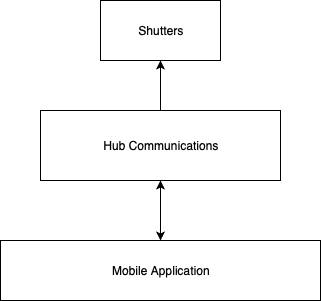
\includegraphics[width=0.60\textwidth]{images/High_Level}
 \caption{A simple architectural layer diagram}
\end{figure}

\subsection{Application Layer Description}
The application layer will take user inputs and send that input to the hub or the shutters directly depending on the connection type. The application layer is also able to request data from the shutters as well such as the current position and battery level 

\subsection{Hub Layer Description}
The Hub will take input from both the app and shutters and reciprocate the information to the intended destination. The commands sent by the app will tell the hub which shutter to interact with and the intended position of the shutter. The hub will also be receive information about each shutters current position and battery level and relay this information to the application

\subsection{Shutter Layer Description}
This layer will process input about changes to the shutters position and then update the shutters to that intended position. This layer would also send out information about the shutters current position and battery level to the application